\chapter{Gesture recognition}
\label{chap:gesture-recognition}

Gesture recognition is a complex topic in computer vision, trying to detect and interpret human movement, postures and gestures. Normally vision-based gesture recognition is composed of four steps, namely model initialization, tracking, pose estimation and gesture recognition and classification \cite{Moeslund} (see figure \ref{fig:4steps}). These steps are further discussed in the following sections.
\begin{figure}[h!]
\center
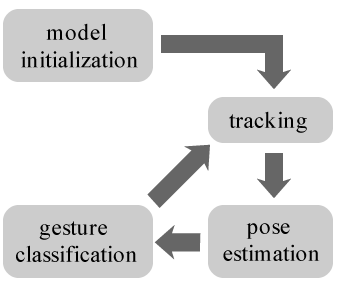
\includegraphics[width=0.3\textwidth]{images/seminar/4steps.png}
\caption{Four main steps in gesture recognition}
\label{fig:4steps}
\end{figure}

%%%-%-%-%-%-%-%-%-%-%-%-%%-%-%-%-%-%-%-%-%-%-%-%%%
%\section{History of gesture recognition}
%\label{sec:history-of-gesture-recognition}

%%%-%-%-%-%-%-%-%-%-%-%-%%-%-%-%-%-%-%-%-%-%-%-%%%
\section{Tracking}
\label{sec:tracking}

The visual tracking techniques in gesture recognition aim at extracting certain features or visual cues for posture estimation and gesture classification. While most of the feature extraction algorithms work principally on images from a single camera \cite{Schmidt}, many setups nowadays use stereoscopic vision from two or more cameras \cite{Chien, VandenBergh}. The depth information gained from stereoscopic vision helps to surpass the big challenge of tracking body parts that are self-occluding in a monocular setting. But stereoscopic vision still has the disadvantage of requiring higher processing speed of the hardware \cite{Schmidt}. %monocular->3dmodel

While most tracking techniques described in this section can be applied in other computer vision problems or gesture recognition applications, which focus on other body parts such as arms, faces or torso, they are also relevant for the gesture recognition topic of tracking hands.

In gesture recognition, tracking mainly consists of the two processes of \textit{figure-ground segmentation} and finding \textit{temporal correspondences} \cite{Moeslund}. Moeslund et al further classify the figure-ground segmentation into five categories: background subtraction, motion based, appearance based, shape based and depth based segmentation.

%------------------------------------------------%
\subsection{Figure-ground segmentation}
\label{sub:figure-ground-segmentation}

\subsubsection{Background segmentation}
The simplest way to separate background from foreground is to take the difference of an empty reference background image and an arbitrary frame. However, this approach is not used, because pixels aren't independent and time-varying background objects should also be considered as background.

In PFinder, Wren et al. \cite{Wren} represented (see figure \ref{fig:pfinder}) each pixel by a Gaussian described by a full covariance matrix, where each pixel is updated recursively with the corresponding statistical properties. This allowed for changes in the background scene like waving curtains or moving objects. The pixels belonging to the figure can then be determined by the Mahalanobis distance. %Moeslund et al. mention that the idea of the mixture of Gaussians (MoG) was introduced by \cite{354}. 
But often the part that needs to be tracked is just a hand or the head in order to further refine a search area. In this case a color cue can be obtained by the same methods.
\begin{figure}[h!]
\center
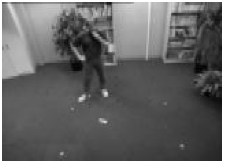
\includegraphics[width=0.4\textwidth]{images/seminar/pfinder1.png}
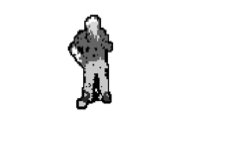
\includegraphics[width=0.4\textwidth]{images/seminar/pfinder2.png}
\caption{Background segmentation in PFinder \cite{Wren}}
\label{fig:pfinder}
\end{figure}

\subsubsection{Motion based segmentation}
Motion based segmentation does not find temporal correspondences but inspects the difference of two consecutive frames, like Sidenbladh did for the figure-ground segmentation of sequences containing a walking figure \cite{Sidenbladh}. Azoz et al. detect time varying edges as a motion cue to separate edges belonging to the figure from edges in the background.

\subsubsection{Appearance based segmentation}
Using the fact that the appearance of the searched body part can vary from person to person, but is definitively different from the appearance of the background, classifiers can be trained with sets of images containing the appearance of positives and sets with negatives for the background. These classifiers can then be used to detect that type of figure in the scene. Usually, this technique gives no figure-ground segmentation but indicates the location in the scene with a bounding box. 

\subsubsection{Shape based segmentation}
Shape based segmentation often refers to silhouette based segmentation which relies on a good background subtraction. Agarwal and Triggs use silhouettes, because they are easily obtained and because shadowing in the figure, clothing and texture is not encoded in the information. But silhouettes have several disadvantages like occlusion problems or shadow attachments that can distort the shape. 
Takahashi et al. \cite{Takahashi} and Chu and Cohen \cite{Chu} also extract shape from multiple cameras to construct a visual hull of the figure. But shape based segmentation is not always silhouette based: Mori et al. use shapes obtained by edge detection \cite{Mori-a} and in \cite{Mori} by a normalized cuts segmentation in order to identify \textit{salient} limbs \ref{fig:normalizedcuts}, which are later assembled into a posture. Azoz et al. use shape filters to detect clusters of colors \cite{Azoz}. 
\begin{figure}[h!]
\center
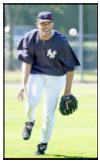
\includegraphics[width=0.2\textwidth]{images/seminar/normalizedcuts1.png}
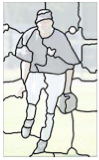
\includegraphics[width=0.2\textwidth]{images/seminar/normalizedcuts2.png}
\caption{Normalized cuts segmentation \cite{Mori}}
\label{fig:normalizedcuts}
\end{figure}

\subsubsection{Depth based segmentation}
Using two ore more cameras, a depth map or a complete three-dimensional reconstruction can be estimated. A depth map \ref{fig:depthmap} can be computed with a disparity map, which is obtained by a correspondence algorithm. Due to the estimation, occlusions or lens geometry problems, depth maps do not always reflect the 3D scene accurately. In \cite{Chien}, Chien et al. refines the accuracy of the correspondence algorithm with epipolar geometry, using the pointing direction from several images.
In \cite{Chu,Takahashi,VandenBergh} silhouettes of the figure from multiple cameras are used to obtain a three-dimensional visual hull with a voxel reconstruction algorithm.
\begin{figure}[h!]
\center
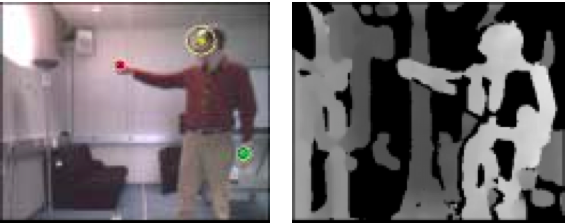
\includegraphics[width=0.8\textwidth]{images/seminar/depthmap.png}
\caption{Scene with estimated depth map \cite{Nickel}}
\label{fig:depthmap}
\end{figure}

%------------------------------------------------%
\subsection{Temporal correspondences}
\label{sub:temporal-correspondences}

Finding the temporal correspondences resolves ambiguities while tracking objects or figures in an image, given their states in past frames. Temporal correspondences can help, when multiple tracked objects occlude each other,  or simply to correctly distinguish two nearby objects.

Commonly, the task of tracking objects across frames is done with an estimator, which first predicts the location of the object for the next frame, based on previous tracking results and secondly reconciles the measured location of the object with the predictions. A broader class of estimators called condensation algorithms, on which the particle filters are based, can also take occlusions into account by representing multiple possibilities as hypotheses or "particles" to predict future locations of the tracked objects.

Schmidt and Fritsch use a kernel based particle filter \cite{Schmidt}, which has the advantage over standard particle filters of avoiding a huge number of particles required for tracking the upper body and arms with 14 degrees of freedom.

%%%-%-%-%-%-%-%-%-%-%-%-%%-%-%-%-%-%-%-%-%-%-%-%%%
\section{Pose estimation}
\label{sec:pose-estimation}

Once the searched limbs or figure features are tracked, pose estimation or model matching adds a layer of abstraction by assembling features into a superstructure which can later be classified. The main goal of pose estimation is to recover an underlying skeletal structure. Moeslund et al. propose a separation of pose estimation methods according to their use of a model \cite{Moeslund}:

%------------------------------------------------%
\subsection{Model-free}
\label{sub:model-free}

Model-free methods do not use a-priori knowledge of the body configuration. The limb or parts are either assembled dynamically or their constellation can be matched to a pose by comparing them to a database of examples.

Agarwal and Triggs presented a method which recovered a 3D pose from monocular images without using manually labeled examples or templates nor using a body model. The pose is estimated by inferring joint angles from silhouettes with a Relevance Vector Machine (RVM) regression \cite{Agarwal}

One of the first model-free pose estimations was PFinder \cite{Wren}. Wren et al. dynamically added blobs to the pose, either by contour matching or a color splitting process. 

Another approach is to dynamically decompose a visual hull into 3D Haarlets (see figure \ref{fig:haarlet}) using Linear Discriminant Analysis (LDA) \cite{VandenBergh} or into shape descriptor atoms with a matching pursuit algorithm and Singular Value Decomposition (SVD) resulting in shape descriptors with the largest eigenvalues \cite{Chu}. Both methods have a key advantage: the atomic shape description and the 3D Haarlets have an additive property (see figure \ref{fig:visualhull}), drastically reducing the number of possible poses to which the measured visual hull can be matched.
\begin{figure}[h!]
\center
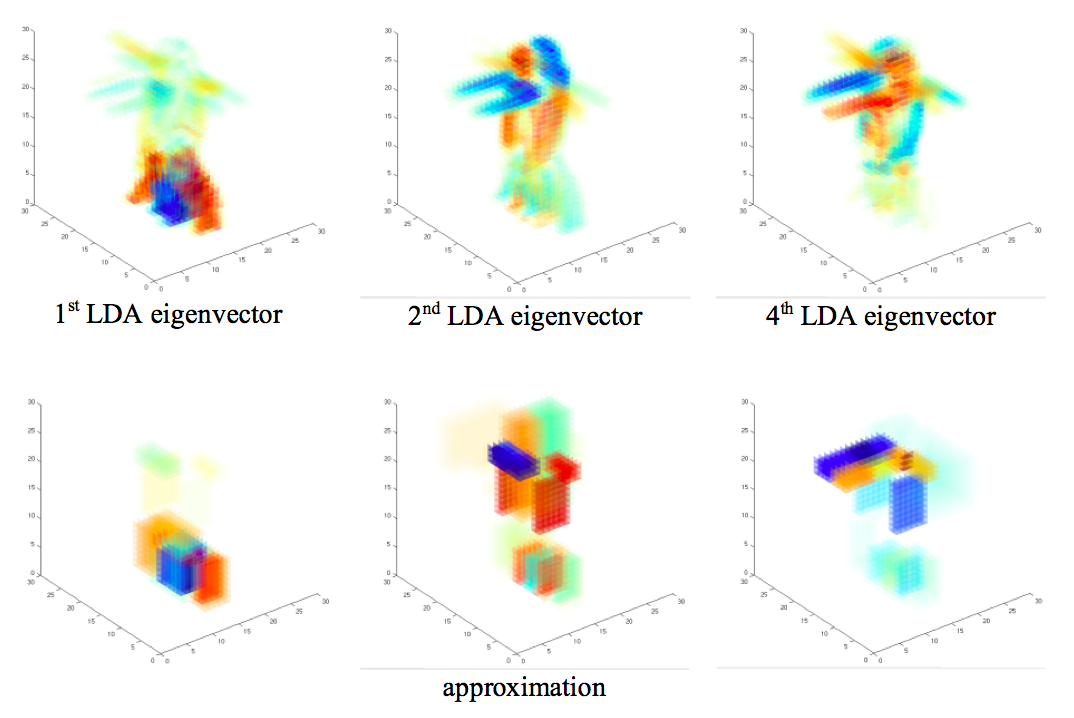
\includegraphics[width=0.8\textwidth]{images/seminar/ldaeigenvectors.png}
\caption{3D Haarlets and their approximation\cite{VandenBergh}}
\label{fig:haarlet}
\end{figure}
\begin{figure}[h!]
\center
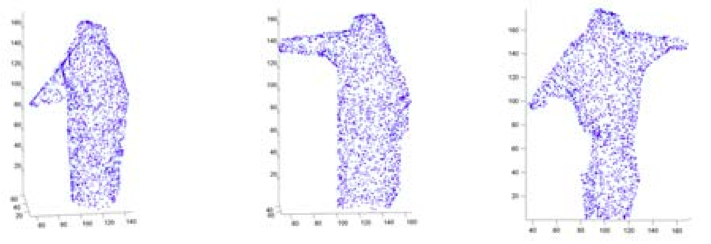
\includegraphics[width=0.8\textwidth]{images/seminar/visualhullcomposition.png}
\caption{Additive property of visual hulls \cite{Chu}}
\label{fig:visualhull}
\end{figure}

%------------------------------------------------%
\subsection{Indirect model use}
\label{sub:indirect-model-use}

This category does not directly map the tracked information onto a model, but rather guides the interpretation. Information like joints, limb length ratios, etc. is labelled into the examples.

Mori et al. use multiple constraints like torso length ratio, adjacency to torso or joints and a-priori body configuration and clothing properties \cite{Mori}. In another approach Mori et al. recover the pose from labelled silhouette examples by deforming the measured shape and therein the skeletal structure to match the labelled example \cite{Mori-a} (see figure \ref{fig:deformable}).
\begin{figure}[h!]
\center
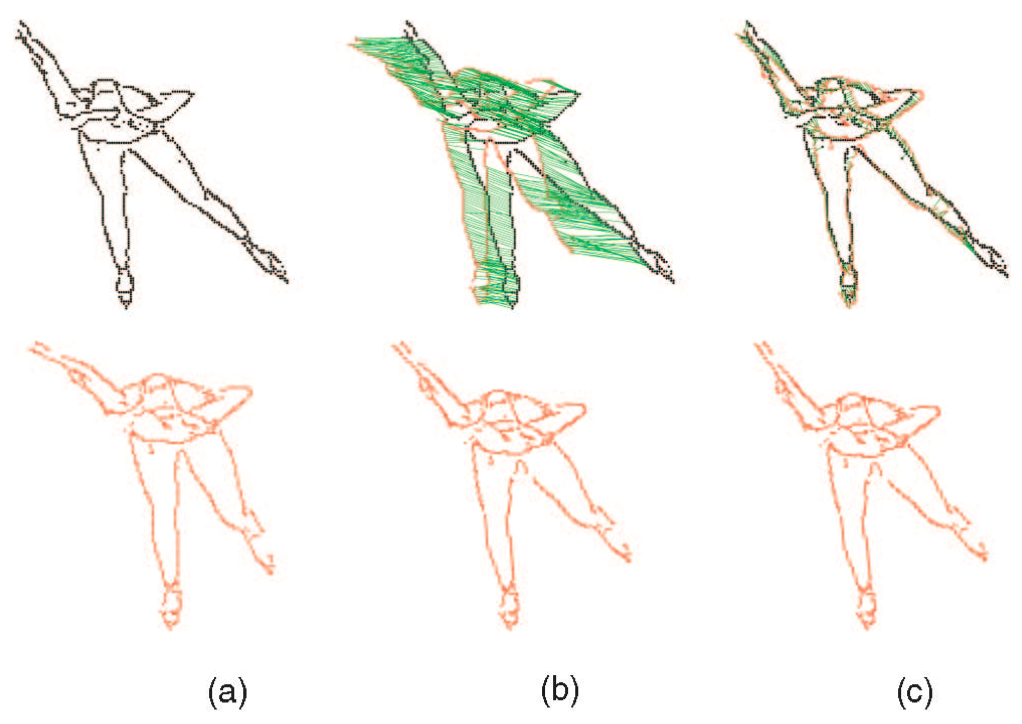
\includegraphics[width=0.8\textwidth]{images/seminar/shapecontextmatching.png}
\caption{Deformable shape context matching \cite{Mori-a}}
\label{fig:deformable}
\end{figure}

%------------------------------------------------%
\subsection{Direct model use}
\label{sub:direct-model-use}

With the direct model approach, the geometric representation of the figure is known beforehand, and the measured data is matched against the model. In newer approaches the model contains human motion constraints to further eliminate ambiguities.

Bray et al. use a smart particle filter (SPF) to fit the tracked results on to a hand model with 15 degrees of freedom and modelling the hand surface in 3D \cite{bray} while respecting the physical model constraints. 
\begin{figure}[h!]
\center
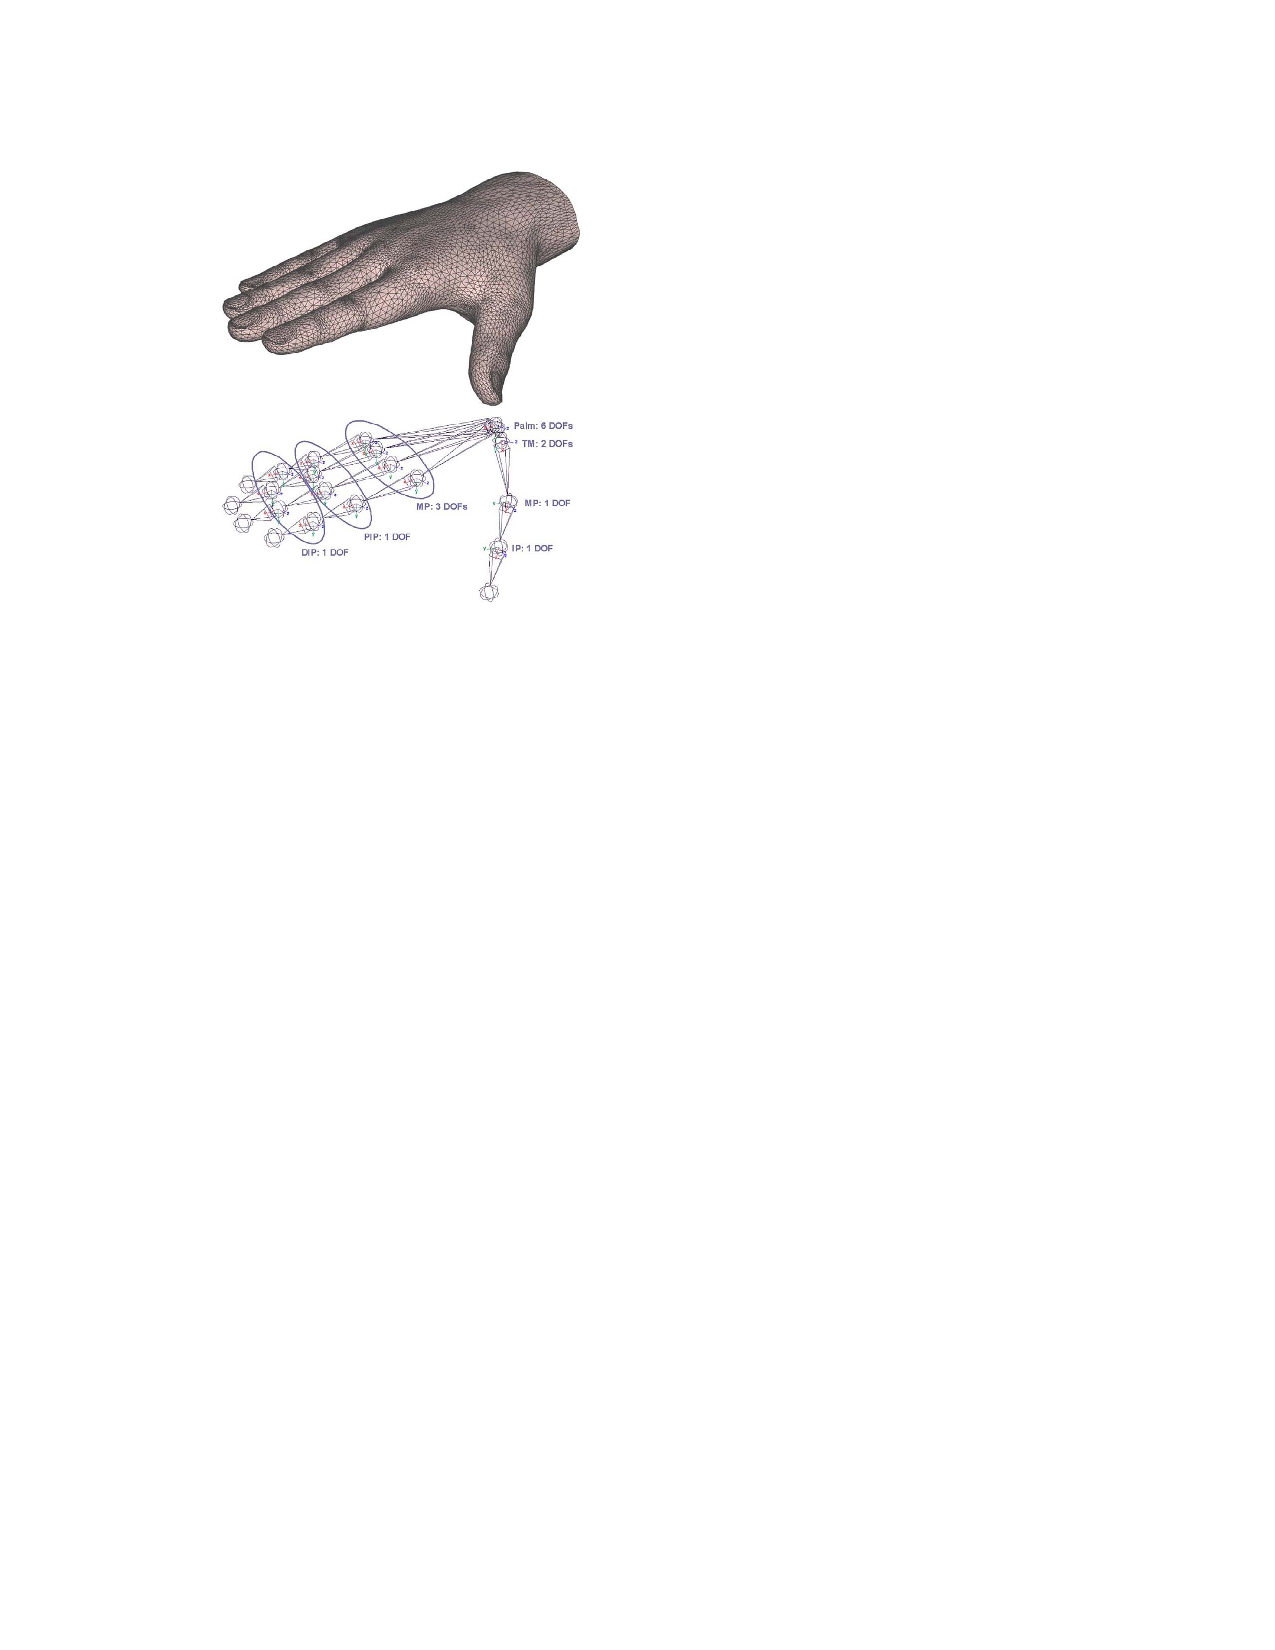
\includegraphics[width=0.5\textwidth]{images/bray_gool_handmodel}
\caption{Hand model as polygonal surface and its skeleton with 15 degrees of freedom \cite{bray}}
\label{fig:bray-gool-hand}
\end{figure}

%%%-%-%-%-%-%-%-%-%-%-%-%%-%-%-%-%-%-%-%-%-%-%-%%%
\section{Recognition}
\label{sec:recognition}

There are several approaches to classify gestures, depending on what information to classify. Because gestures can be viewed as sequence of postures in time, the most widely used classification method is a Hidden Markov Model (HMM). HMMs are suited for the classification of gestures, they try to model the spatio-temporal variability and to maximize the likelihood of generating all examples of a gesture class \cite{Yang}.
 
Yang et al. trained a HMM for spotting specific body gestures like raising a hand, jumping etc., but also presented the concept of the garbage gesture model (see figure \ref{fig:garbage}) and the key gesture spotting model (see figure \ref{fig:gesturespotter}). The garbage gesture model is an ergodic model and tied in the the key gesture spotter model at the beginning of a gesture and at the end \cite{Yang}.
\begin{figure}[h!]
\center
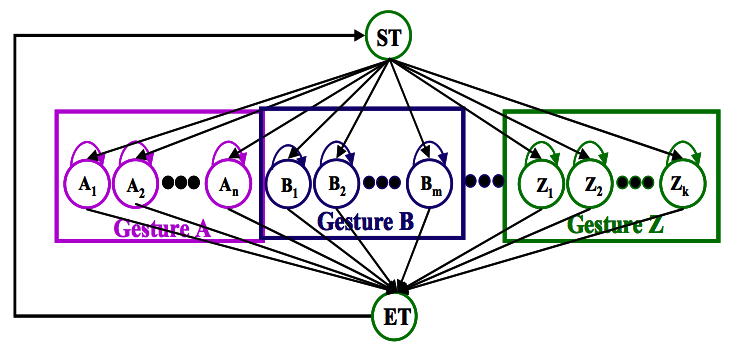
\includegraphics[width=0.5\textwidth]{images/seminar/garbage.png}
\caption{Garbage gesture model \cite{Yang}}
\label{fig:garbage}
\end{figure}
\begin{figure}[h!]
\center
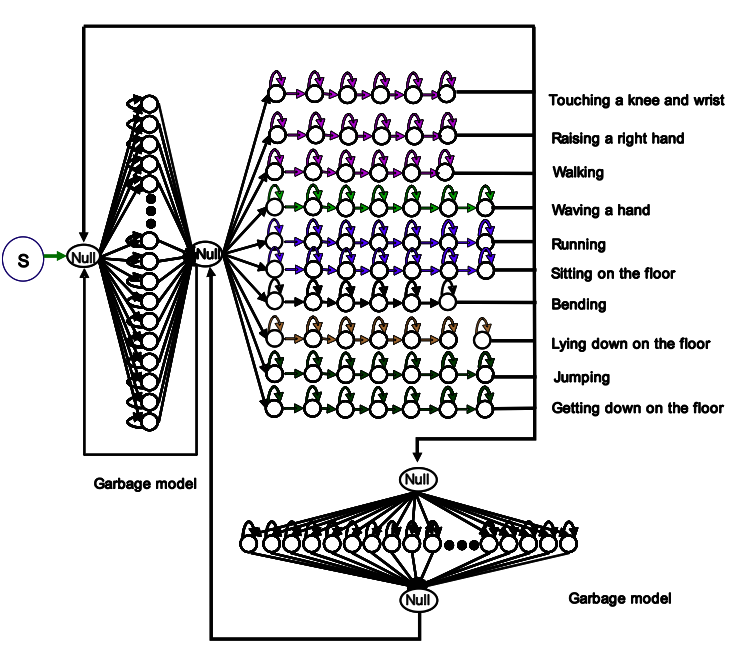
\includegraphics[width=0.6\textwidth]{images/seminar/gesturespotter.png}
\caption{Key gesture spotter model \cite{Yang}}
\label{fig:gesturespotter}
\end{figure}

Both Willson et al. and Chu and Cohen used the concept of a multiphasic gesture: in a sequence of postures, there is at least a transition to the key posture and a transition leaving it. Gestures can also have several key postures identifying a gesture. While Willson et al. did not use hidden states but a simpler markovian chain, Chu and Cohen used a dual-state HMM for a primary and secondary decomposition of gestures, which also gives smaller set of atoms and a HMM state space of linear complexity \cite{Chu,Wilson}.

Wang et al. introduce a powerful approach for gesture classification: hidden conditional random fields (HCRF) (see figure \ref{fig:hcrf}). HCRFs incorporate hidden states variables in a discriminative multi-class random field. It is an extension of the spatial Conditional Random Fields and takes the main advantage of HMMs, the capability of modelling temporal sequences. HCRFs can be used like HMMs (see figure \ref{fig:hmm}), but the hidden states can be shared among different gesture classes \cite{Wang}. 
\begin{figure}[h!]
\center
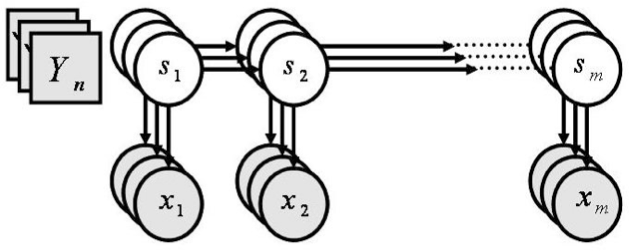
\includegraphics[width=0.45\textwidth]{images/seminar/hmm.png}
\caption{Hidden Markov Model \cite{Wang}}
\label{fig:hmm}
\end{figure}
\begin{figure}[h!]
\center
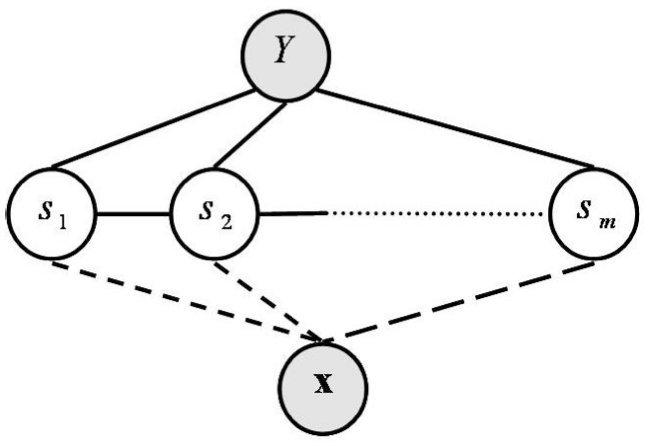
\includegraphics[width=0.3\textwidth]{images/seminar/hcrf.png}
\caption{Hidden Conditional Random Field \cite{Wang}}
\label{fig:hcrf}
\end{figure}

%\subsection{Hidden markov models}
%\label{sub:hidden-markov-models}

%\subsection{Bayesian networks}
%\label{sub:bayesian networks}

%%%-%-%-%-%-%-%-%-%-%-%-%%-%-%-%-%-%-%-%-%-%-%-%%%
%\section{Current development}
%\label{sec:current-development}

%After this general overview of the steps generally used in gesture recognition, the field of hand recognition has something something.

%particlefilter
%->mit

\section{Our approach}
\label{sec:our-approach}

Erol et al. \cite{hand-review} mention the difficulties in hand gesture recognition: 
\begin{itemize}
\item high-dimensional problem
\item self-occlusion
\item uncontrolled environment
\item rapid hand movements
\item processing speed
\end{itemize}
There is an approach from Wang and Popovic from MIT, where the processing requirements are circumvented by generating a nearest neighbours lookup database for scaled-down 40$\times$40 pixel images of a color marked glove (see figure \ref{fig:mit}) \cite{mit}.
\begin{figure}[h!]
\center
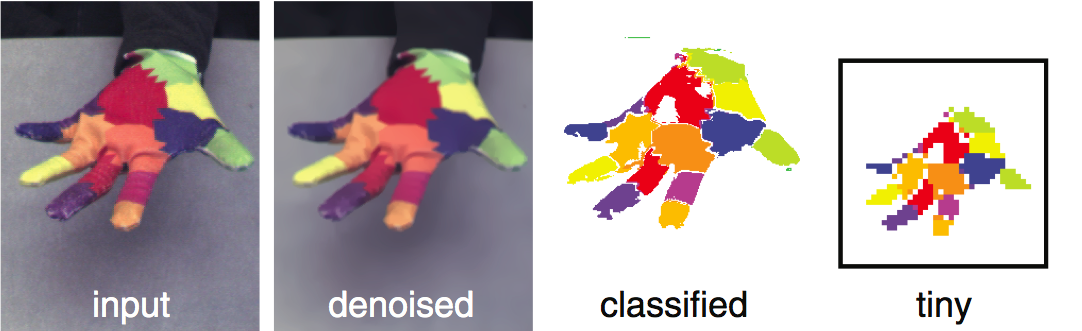
\includegraphics[width=0.6\textwidth]{images/mit}
\caption{Pose estimation with a color-marked glove and its 40$\times$40 pixels representation (tiny) \cite{mit}}
\label{fig:mit}
\end{figure}

However many tracking algorithms widely used in gesture recognition are confronted with real-time problems. Preliminary tests with advanced algorithms have been done in OpenCV \cite{opencv} -- a computer vision library that includes over 500 algorithms from research -- using optical flow algorithm or background subtraction with mixtures of gaussians. While the results are real-time capable for smaller images, the frame-rate often drops to under 10 frames per second for bigger images.

Our approach aims at using simple techniques focusing on speed with some constraints limiting the scope of the project and still having an architecture where an real-time ergonomic gestural  interface is possible.
%realtime focus